
\section{Design}
\label{sec:design}

\subsection{External factor collection}
\label{subsec:external}
Sensing module is mainly designed for collected the external factors of users.

\paragraph{Food intake}
As the food intake is a main source of carbohydrate, \sysname provides the food menu for users to record their daily intakes based on the carbohydrate food list \cite{bib:carblist}.
Five common food categories have been provided by \sysname, including grains ,vegetables, mike and egg,fruits and meats. The users are asked to enter their food items and the corresponding amounts. \sysname calculate the carbohydrate of a meal and measure its impact on blood glucose level.

\paragraph{Drug intake}
The oral diabetes medications enhance secretion of insulin into the blood by the pancreas or decrease amount of glucose released from liver, keeping the blood glucose in a low level for type II diabetes.
In \sysname, a drug menu of 11 oral diabetes is report for users to input their drug intake. After eating the diabetes drugs, users select their pills name and report the drug dosage. The drug list is provided based on \cite{bib:druglist}.
\sysname transfers the drug dose as the blood glucose efforts according to their work functions \cite{bib:druglist, bib:bolen2007systematic, bib:bennett2011oral}  by physiological model.

\paragraph{Insulin injection}
Insulin injection is to control blood glucose concentration of those who have type I diabetes, and the patients of type II, whose blood sugar is too high for their bodies to control. \sysname provides a insulin type list based on \cite{bib:insulinlist} for user with diabetes to enter their usage and insulin dosage, and then transfer it into physiological model to compute the blood glucose level.

\paragraph{Activity factors}
Since the carbohydrate in the body can be consumed by daily exercise, resulting to varying the blood glucose level, \sysname adopts an effective and power efficient approach \cite{bib:kwapisz2011activity} to automatically recognize six common user's daily activities (i.e., walking, running, upstairs, downstairs, sitting and standing), and record the corresponding durations. The caloric expenditure can be easily consumed by the calorie burn calculator formulas as Equation ~\ref{calorie_burn}.
\begin{equation}\label{calorie_burn}
  Calorie Burn = (BMR/24)*MET*T,
\end{equation}
where BMR (Basal Methobolic Rate) is the amount of energy required to simply sit or lie quietly \cite{bib:mcnab1997utility}, and MET (Metabolic Equivalent) is the ratio of the work metabolic rate to the resting metabolic rate\cite{bib:ainsworth2000compendium}. The calculator formula has been widely used by multiple sport applications \cite{bib:shapesense, bib:HealthStatus, bib:CalorieCounter}.
\sysname finally leverages the calories to measure the effects of exercise on the blood glucose.

\paragraph{Sleep quality}
Sleep quality has a long influence on blood glucose level. To measure the sleep quality of users, \sysname applies an effective method in \cite{bib:gu2014intelligent} to measure the sleep quality, and leverages the sleep quality score as an index to evaluate the sleeping impact on blood glucose level.

\subsection{Feature Engineering of Physiological-Temporal Views }
\subsubsection{Physiological View}

\begin{figure}[t]
  \centering
  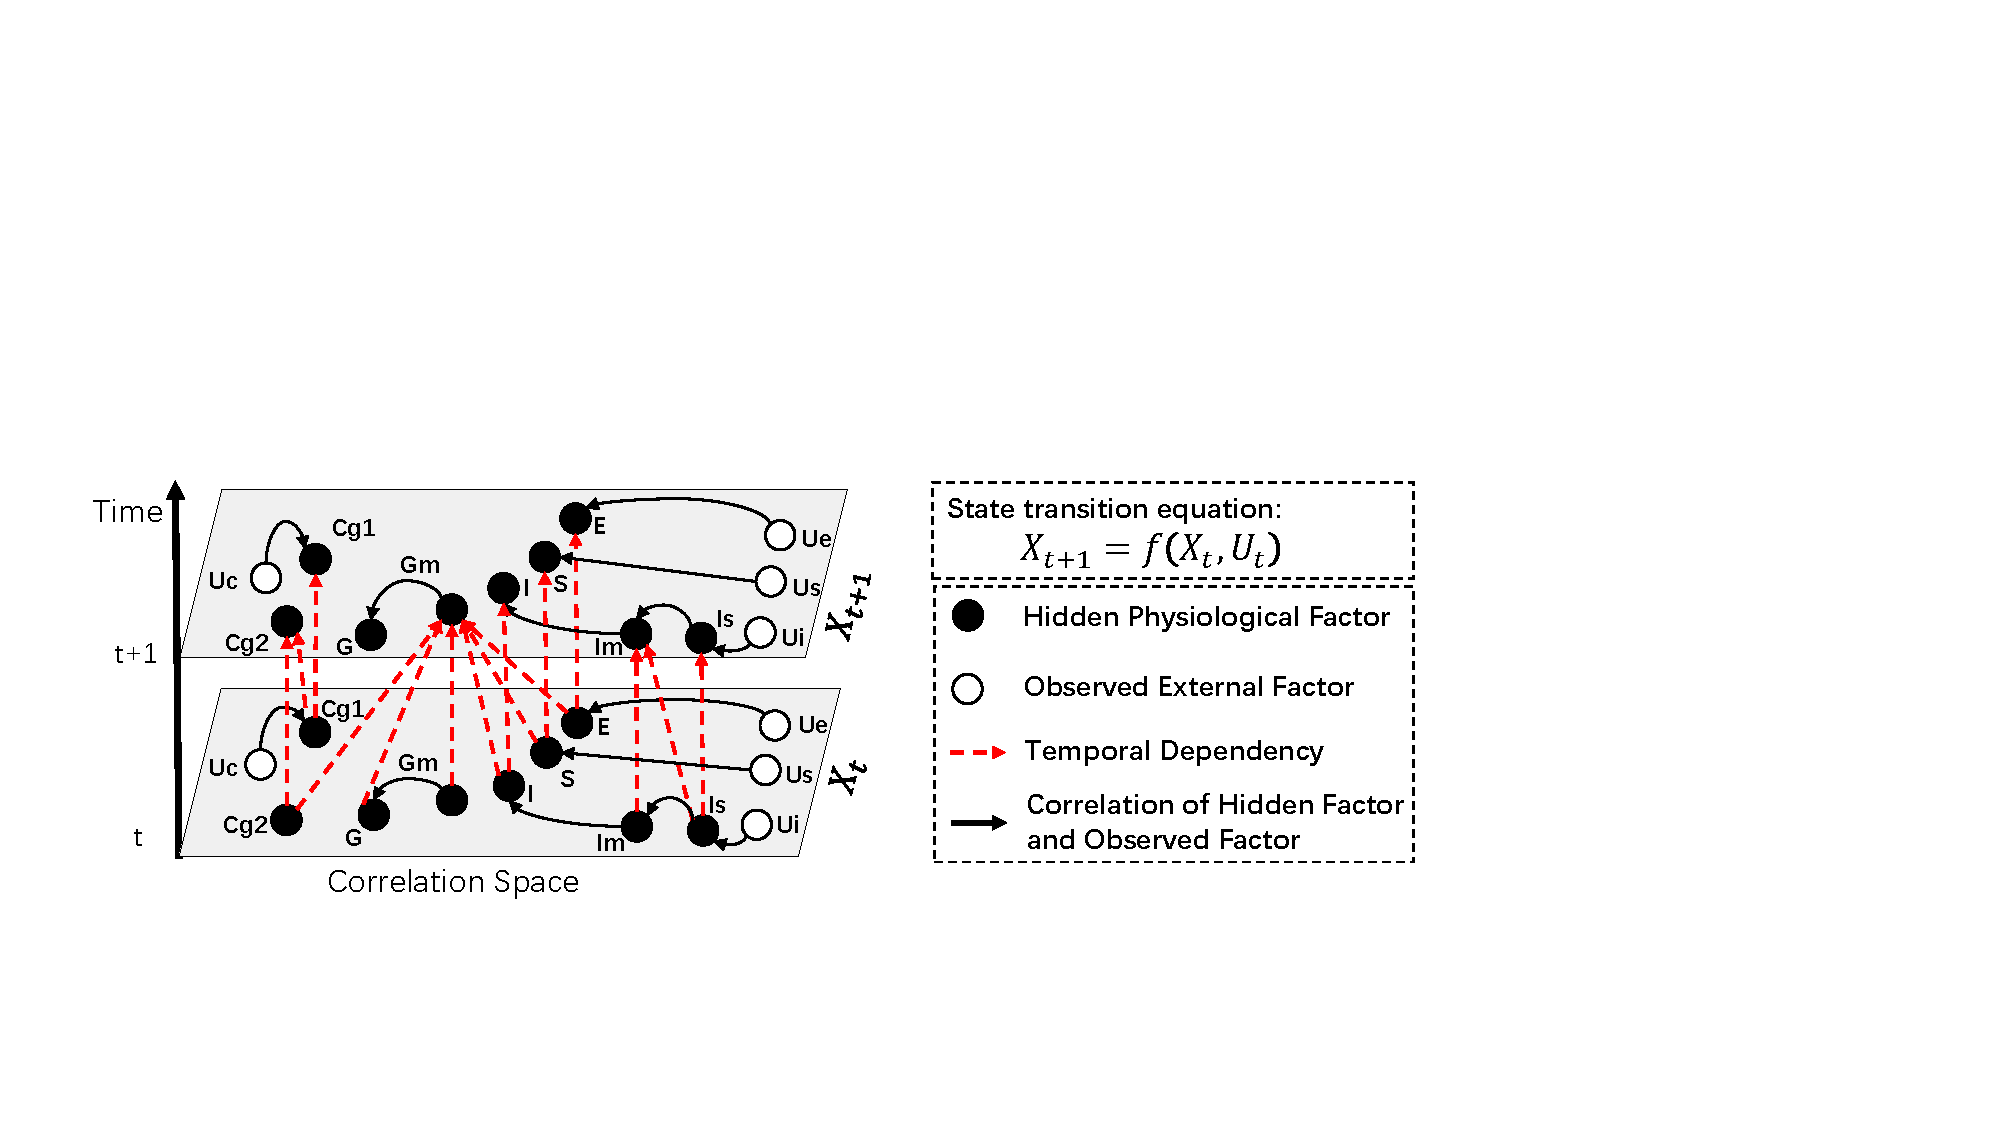
\includegraphics[width=0.9\columnwidth]{./img/Physiological_correlation1.pdf}
  \caption{Temporal graph of the physiological model.}
  \label{fig:phymodel}
\end{figure}
The feature engineering of physiological view is to leverage a physiological model to quantify the dynamics of physiological factors in the body. The 
physiological model, based on the physiology mechanism of blood glucose in Section~\ref{sec:preliminary}, has been widely studied in previous works \cite{bib:briegel2002nonlinear,bib:duke2010intelligent, bib:plis2014machine}.It primarily measures the real-time values of carbohydrate, insulin and glucose influenced by the external factors. We constructed our physiological model based on the work \cite{bib:duke2010intelligent},
with an extension of sleeping fact according to its physiological impact discussed in Section~\ref{sec:preliminary}.

\paragraph{Temporal Graph of Physiological Model}
Given the hidden physiological vectors $X_{t}=\{C_{g1}(t), C_{g2}(t),\\ I_{s}(t),I_{m}(t), I_{t}, G_{m}(t), G(t), E(t)\}$, where the elements of this vector represent
the hidden physiological factors at time point $t$, and the observable input vector $U_{t}=\{U_{c}(t), U_{e}(t), U_{s}(t), U_{i}(t)\}$ , in which $U_{c}$ stands for the 
carbohydrate proportion of meals, $U_{e}$ indicates the calories cost by exercise,  $U_{s}$ is the sleep score and $U_{i}$ states for the amount of insulin injected or simulated 
by the diabetes drugs  at time point $t$. In particular, the sleep quality $U(s)$ is a constant during a whole day.
The station transition functions can be represented as $X_{t+1}=f(X_t, U_t)$, and its corresponding
temporal transition graph is shown as \figref{fig:phymodel}.  %\tabref{phy_tab} details the transformation functions of the carbohydrate $C_{g1}$ and $C_{g2}$, and insulin

%As \figref{fig:phymodel} shown, the equations of $C_{g1}$ (Equation~\ref{Eq:Cg1}) and $C_{g2}$ (Equation~\ref{Eq:Cg2}) indicating the temporal transitions of carbohydrate consumption and the carbohydrate digestion respectively.   

In detail, $C_{g1}$  and $C_{g2}$ indicate the carbohydrate consumption and the carbohydrate digestion respectively, and their transition equations are shown 
in Equation~\ref{Eq:Cg1} and Equation~\ref{Eq:Cg2}.

\begin{equation}\label{Eq:Cg1}
C_{g1}(t+1)=C_{g1}(t)-\alpha_{1}^c*C_{g1}(t)+U_{c}(t)
\end{equation}

\begin{equation}\label{Eq:Cg2}
C_{g2}(t+1)=C_{g2}(t)+\alpha_{1}^c*C_{g1}(t)-\alpha_{2}^c*C_{g1}(t)
\end{equation}

The equations of $I_{s}$ (Equation~\ref{Eq:Is}) and $I_{m}$ (Equation~\ref{Eq:Im}) showing the temporal transitions of  the subcutaneous insulin
and the insulin mass respectively. $I$, the level of active plasma insulin, can be achieved by Equation~\ref{Eq:I}, where $S^I$ and $bm$ refer to the 
insulin sensitive and body mass respectively. 
\begin{equation}\label{Eq:Is}
I_{s}(t+1)=I_{s}(t)-\alpha_{f}^I*I_{s}(t)+U_{I}(t)
\end{equation}


\begin{equation}\label{Eq:Im}
I_{m}(t+1)=I_{m}(t)-\alpha_{f}^I*I_{s}(t)-\alpha_c^I*I_{m}(t)
\end{equation}

\begin{equation}\label{Eq:I}
I(t)=\frac{I_{m}(t)*S^I}{142*bm}
\end{equation}

$E$ denotes the exercise effect on insulin over the past time window. This long-term influence can be 
expressed by a cumulative moving average as Equation~\ref{Eq:E} in the physiological model. 

\begin{equation}\label{Eq:E}
E(t-t_0+1)=(t-t_0)*E(t-t_0)+U_{e}(t-t_0)
\end{equation},

where $t$ and $t_0$ are the current and beginning time point in the past time window. In \sysname, 
the window size of exercise is set to 24 hours, which optimizes the experimental results and matches the conclusion
of clinical studies. 

$S$ represents the sleeping quality effect on insulin. In physiological model, sleeping 
effect also maintains a long-term influence on the insulin as the exercise effects,
and is shown as Equation~\ref{Eq:S}.

\begin{equation}\label{Eq:S}
S(t-t_0+1)=(t-t_0)*S(t-t_0)+U_{s}(t-t_0)
\end{equation},

where $t$ and $t_0$ are the current and beginning time point in the past time window. In \sysname,
the window size of sleep lasts for 7 days, which optimizes the experimental results and matches the conclusion
of clinical studies.

Based on the positive factors and the negative factors, the blood glucose mass of individual body 
$G_m$ can be calculated as Equation~\ref{Eq:Gm}
\begin{equation}\label{Eq:Gm}
G_m(t+1)=G_m(t)+\delta_{abs}-\delta_{ind}-\delta_{dep}-\delta_{clr}+\delta_{egp}
\end{equation},
where $\delta_{abs}=\frac{\alpha_3^c*\alpha_2^c}{1+25/C_{g2}}$

and the blood glucose concentration $G$ can be computed in Equation~\ref{Eq:G}.
\begin{equation}\label{Eq:G}
G_m(t+1)=G_m(t)+\delta_{abs}-\delta_{ind}-\delta_{dep}-\delta_{clr}+\delta_{egp}
\end{equation},

 
1) Positive factors:
Positive factors indicates the

However, the parameters of this model are different to individuals and also hard to be tuned.

\subsection{Blood glucose level prediction}

% !TEX root = paper.tex

\subsection{Intuition}
Given the features extracted from the physiological process, it seems plausible to perform any classification algorithm for blood glucose level prediction. Nonetheless, this plug-and-play approach will neglect important information from (1) dynamics of the process, and (2) inter-user similarity among same group of participants. Traditionally, various sequential classification methods[], e.g., hidden Markov model (HMM), recurrent neural networks (RNN), and dynamic conditional random fields (CRF), are used to capture the temporal correlation of the input feature. The inter process correlations are often times incorporated with the so-called multi-task learning approaches[], which learns processes (or tasks) in parallel to improve classification or to reduce the data sample requirement. 

In this paper, a novel machine learning paradigm, namely Multi-division deep-dynamic RNN (Md$^3$RNN), is proposed. To include the the aforementioned information sources in an unified framework, we develop two key ideas that extend the classical RNN. Firstly, the single hidden layer in RNN is replaced with several deep stacked layers. The deep structure in the new model is able to describe complex, mutli-scale system dynamics that would otherwise be ignored (or averaged out) by prior ``shallow'' models such as HMM, RNN, and CRF. Secondly, the correlations among users, being quite significant within user groups (divisions), are encoded by group-shared input layer and common hidden layers, whereas the distinct characteristics of individual users are modeled with  different output layers for personalized prediction. Within a larger scope of machine learning, the proposed Md$^3$RNN aims to leverage recent advancement of deep learning and multi-task learning, to model group-interacted time series data having complex temporal dynamics. It can be viewed as both a deep extension of RNN, and an intermediate between single-task learning and multi-task learning, hence the name Md$^3$RNN.

The overall configuration of the proposed model is summarized in Fig.\ref{fig:rnn}. Detailed construction of each component is given in the sequel.     

\begin{figure}[!t]
  \centering
  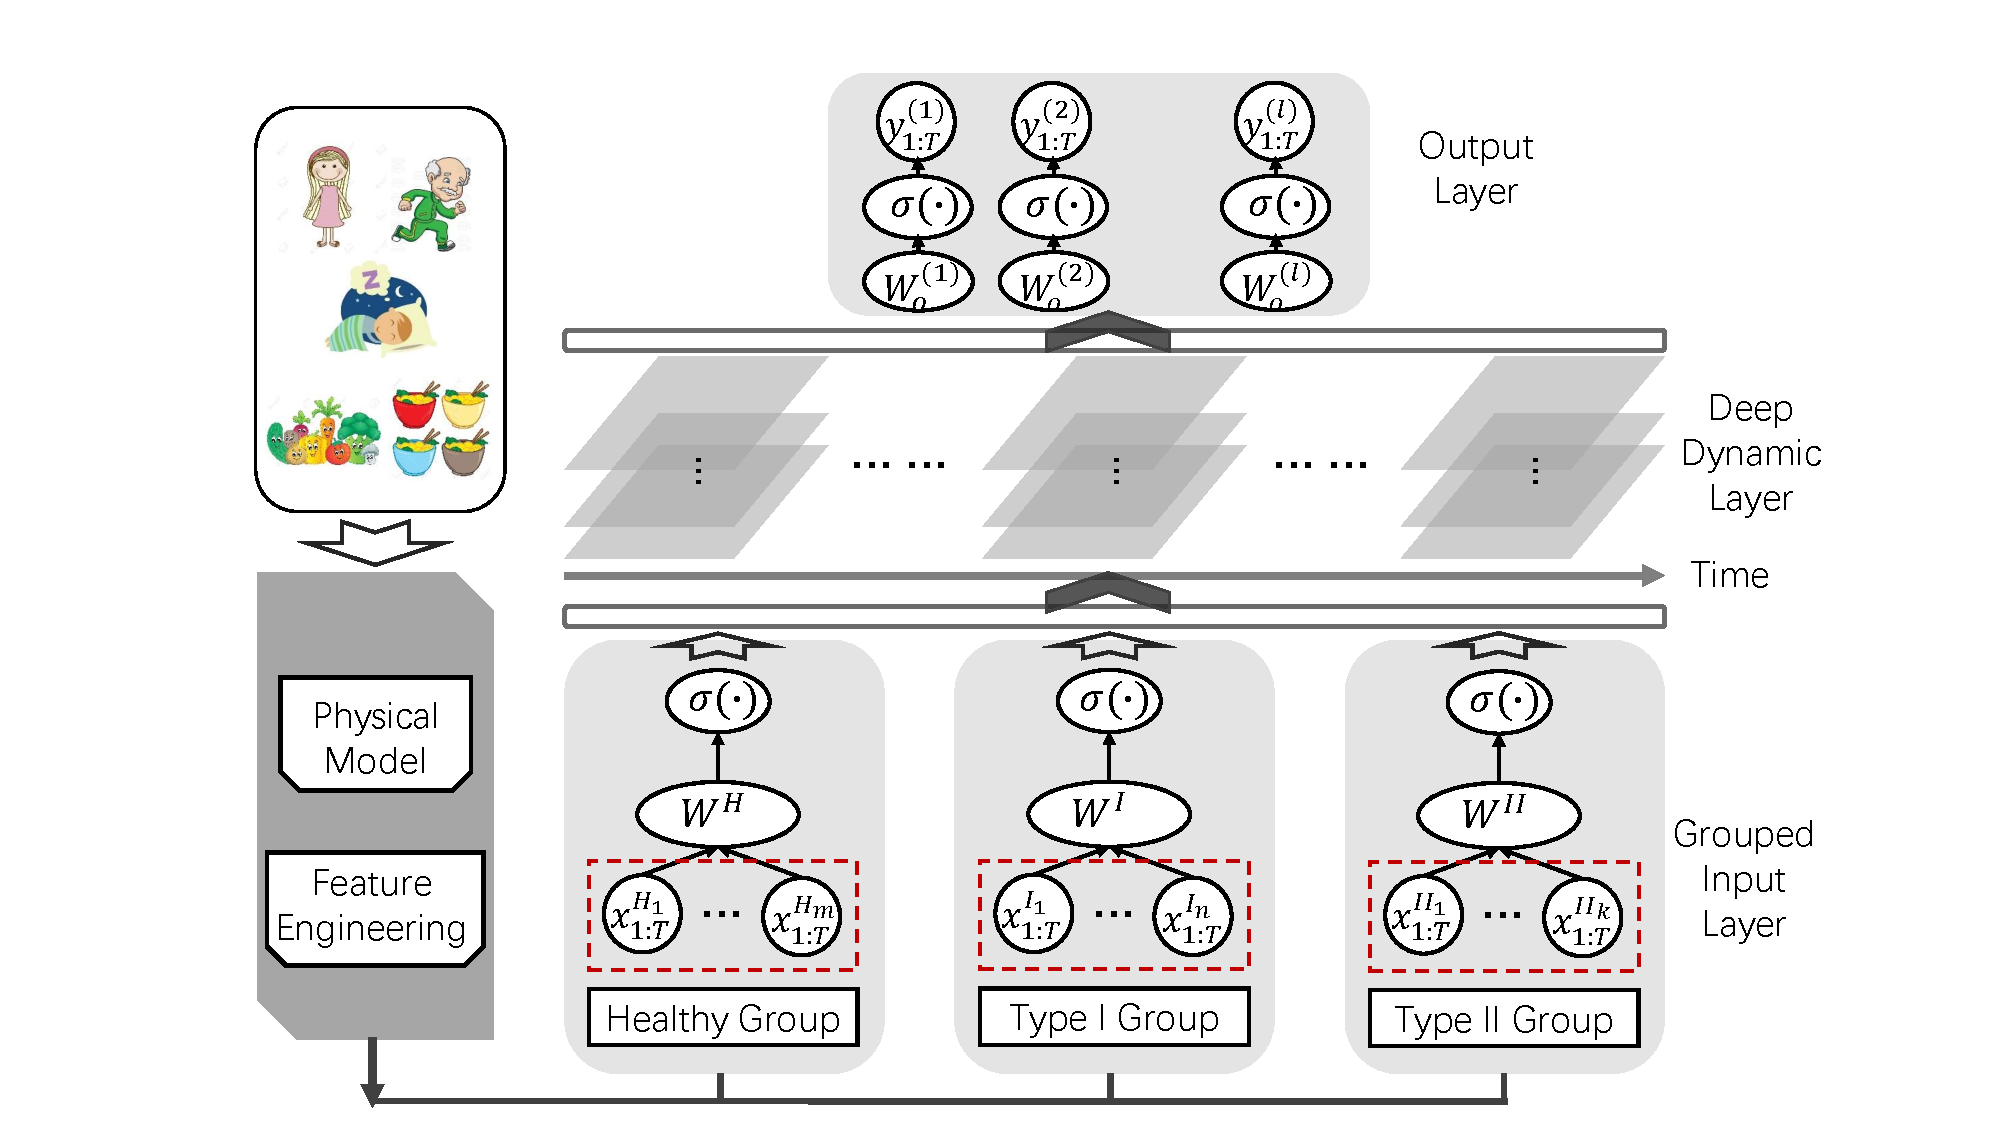
\includegraphics[width=0.9\columnwidth]{./img/pics_RNN.pdf}
  \caption{The Md$^3$RNN structure}
  \label{fig:rnn}
\end{figure}

\subsection{Model construction by layers}
The input of the Md$^3$RNN are the features extracted from the physiological model. The labeled data sequences for user number $j$ at time $t$ are denoted by $(x_i^{j},y_i^{j})$. We also adopt an index set convention, that $(x_A^{B},y_A^B)$ represents the data set $\left\{(x_i^{j},y_i^{j}) | i \in A, j\in B\right\}$ given index sets $A$ and $B$.
\subsubsection{Grouped Input Layer}
In the context of blood glucose prediction, available inputs are naturally divided into three groups according to the health condition of the participant from whom the data was generated. Notation-wise, we utilize $H$, $I$ and $II$ to indicate the the group of healthy user, user with type I diabetes and those having type II diabetes, respectively. Since the extracted features are essentially physiological indexes of an ``average'' person, they must go though different transformations to represent useful information of three distinct groups. This consideration motivate the design of the input layer (bottom of Fig.\ref{fig:rnn}) - it is divided into three units that performs different linear and non-linear transformation according to user groups. For instant, a data sample $x_t^{I_j}$, generated at time $t$ from the $j^{th}$ user of type I, undergoes the following processing:
\begin{align}
\tilde{x}_t^{I_j} = \sigma \left( W^Ix_t^{I_j} \right)
\end{align}     
where $W^I$ is the coefficients of the affine transformation \footnote{We assume that the interception is included in $W$. This can be done by simply adding a feature of all $1$s.}, $\sigma$ is some activation function, and $\tilde{x}_t^{I_j}$ is the output of the input layer for that data sample. Similar operations are conducted for data samples from group $H$ and $II$, but with different transformation coefficients. Intuitively, the shared transformation within groups would improve the learning of parameters (vs. single task learning), as information from all data in a homogeneous group is used. Also, the transformation can be stacked into several (say $P$) layers, for better information representation.   

\subsubsection{Deep Dynamic Layer}
A common hidden layer is designated to capture the dynamics of the blood glucose evolution process. The underlying assumption is that, the biological and chemical reactions governing blood glucose variation are similar for all people, despite of grouped behaviors in the representation of physiological indexes (input layer), or individual characteristics in exhibited glucose level. This assumption could be justified by a series of medical research[][]. Moreover, since all users share the same hidden layer, all collected data samples are eventually helping the estimation of its parameters. The availability of rich information for the hidden layer makes the learning of a deep structure possible. In Md$^3$RNN, a number of Long Short Term Memory (LSTM) networks are stacked together (middle of Fig.\ref{fig:rnn}), to increase the overall model flexibility. In particular, it has been justified in both theory and practice that stacked LSTMs are able to capture dynamics occurring at different time scales, which in the current application would enable the modeling of both slow and rapid biological/chemical reactions. Although a wide variety of LSTM configuration exist in literature, in this work we adopt the one recently proposed by [], which combines the forget/input gate and merges cell/hidden state for simplicity and better generalization performance. Mathematically, given the output from the grouped input layer, the deep dynamic layer performs
\begin{equation}
\begin{aligned}
&z^d_t = \sigma\left( W^d_z [h_{t-1}^d,h_t^{d-1}] \right) \\
&r^d_t = \sigma\left( W^d_r [h_{t-1}^d,h_t^{d-1}] \right) \\
&\tilde{h}_t^d = tanh\left( W^d_h [r_t^d*h_{t-1}^d,h_t^{d-1}] \right) \\
&h^d_t = (1-z_t^d)*h_{t-1}^d + z_t^d*\tilde{h}_t^d
\end{aligned}
\end{equation}
for hidden layer numbered $d = 1,2,\cdots,D$. At the first dynamic layer with $d=1$, the input $h_t^{d-1}$ is set to be the output from the grouped input layer, and the output of the last dynamic layer, $h^D_t$, will be used as the input of the last component of Md$^3$RNN. 

\subsubsection{Personalized Output Layer}
Finally, each user is assigned a personalized output layer, parameterized by $W_o^j, j=1,\cdots,l$, which performs a single linear and softmax transformation on the results of the deep dynamic layer. The particular configuration of the output layer compensates for the individual characteristics in the exhibited blood glucose (i.e., measured blood glucose level). Because only data generated by a specific participant $j$ will have an effect on the its parameters $W_o^j$, the personalized output layer is set to have a ``shallow structure'', i.e., it only performs the transformation once. More specifically, given $h^D_t$ from user $j$, it computes
\begin{equation}
\hat{y}_t^j = \text{softmax} \left( W_o^j h^D_t \right)
\end{equation}

\subsection{Cost Sensitive Learning and Hyperparamter (Model) Selection}

Similar to other deep neural network learning, Md$^3$RNN is trained by minimizing the sum of losses over all the time steps. The definition of the loss function has much bearing on the generalization performance of the method. In particular for the current application, simply minimizing a general error rate seems inappropriate, because the costs of different types of misclassifiction errors are not the same. For example, missing the detection of high blood glucose (type I or II) is more costly than misclassifying normal condition to an alarm for high glucose. Moreover, in the collected data set from real people, the training data is inherently imbalanced - the available samples labeled Level 1 and Level 4 are much fewer (only 7\%) compared to samples in the other categories (Level 2 and Level 3). 

The above concerns motivate the cost sensitive learning of Md$^3$RNN. Instead of directly minimizing a surrogate of error rate, we propose to optimize over a weighted version of classification losses[]. More specifically, the following total loss function is considered:
\begin{equation}
L = \sum_{t} \sum_{y_t \in \mathcal{Y}} l(y_t,\hat{y}_t)C_{y_t}
\end{equation} 
where $\mathcal{Y}$ is the label set, and $\hat{y}_t$s are prediction output from Md$^3$RNN. Our implementation uses cross entropy for $l(y_t,\hat{y}_t)$, but generally the ``base'' lost function $l(y_t,\hat{y}_t)$ can be any surrogate of the error function. The additional coefficient $C_{y_t}$ weights the misclassification error for category $y_t$. In the current application, $\mathcal{Y} = \{1,2,3,4\}$, associated with four coefficients $C_1$ to $C_4$. Those cost weighting coefficients are treated as hyperparameters of the proposed model, but in other applications of Md$^3$RNN, they can also be determined with prior knowledge about the misclassification cost and the class imbalance. 

With the technique of back-propagating, computing the gradient of Md$^3$RNN is not so different from gradient calculation of classical RNN. In this work, we accomplish those computation using Tensorflow[], and proceed to learn Md$^3$RNN model by stochastic gradient descent for overall loss minimization.

Last but not least, the construction of the Md$^3$RNN model involves choosing 15 hyperparameters, e.g., cost coefficients $C_{y}$, depth $D$ of the stacked dynamic layer, learning rate, number of hidden unit in the input layer, etc. Direct application of cross validation (CV) for hyperparameter tuning, even with the help of parallel computing, seems endless as the number of required CVs scales exponentially to the number of hyperparameters. In this regards, we adopt Bayesian optimization (BO), a recent tool developed for blackbox function optimization with limited evaluations. The decision variables of BO are those hyperparameters, and the objective is the F-score of the precision and recall on some testing data set. Note that BO has been used recently for the hyperparameter (model) selection of many deep learning paradigms [][].            




